\section{The Diagrammatic Monte Carlo method}
\subsection{The Monte Carlo sampling method}
The Monte Carlo method is not a specific technique, but rather a wide set of similar methods which employ probability to solve problems 
that are otherwise too complex for an analytic solution and too resource demanding to solve with a numerical method.\\
The basic idea behind Monte Carlo is to use a statistical approach in the resolution of difficult integral and differential equations 
\cite{metropolis1949monte} by the means of a precisely defined set of rules and a random number generator.\\
This method is an \textit{iterative stochastic procedure}, or in layman terms, a technique that is iterative: it needs to be applied many times in 
order to produce an extremely large number of measurements from which it is possible to build an estimate for a determined quantity, 
using the \textbf{central limit theorem} and the law of large numbers, and stochastic: it uses random numbers to obtain all sorts of distributions, 
usually through a precisely defined set of rules with a \textbf{Markov chain}.\\
It is in fact possible, using a Monte Carlo method, to estimate the ground state of the time-independent Schroedinger equation \cite{gubernatis2016quantum}
\begin{equation}
    -\nabla^2\psi(x,y,z)=\left[E-U(x,y,z)\right]\psi(x,y,z)
\end{equation}
using the following ansatz for the wavefunction:
\begin{equation}
    u(x,y,z,\tau)=\psi(x,y,z)e^{-E\tau},
\end{equation}
thus introducing a fictitious imaginary time-dependence. In this way $u(x,y,z,t)$ follows the diffusion equation
\begin{equation}
    \frac{\partial u}{\partial \tau}=\nabla^2u-Uu,
\end{equation}
which can be framed in a Monte Carlo representation as a set of weighted particles which independently perform a random walk with an 
exponential decay in imaginary time and a rate governed by the energy eigenvalue $E$, together with a particle distribution which can be used 
to determine an estimate for the wavefunction $\psi(x,y,z)$.\\
Note that the transformation performed on the wavefunction (first done by Fermi) is exactly the already seen transformation used for the Matsubara Green's 
functions \ref{imaginary_time_substitution}, which turns the standard time-dependent Schroedinger equation
\begin{equation}
    i\frac{\partial \psi}{\partial t}=-\nabla^2\psi+U\psi
\end{equation}
into
\begin{equation}
    \frac{\partial\psi}{\partial \tau}=\nabla^2\psi-U\psi.
\end{equation}
This observation already stresses the importance of imaginary time in our computation.
We list three main types of Monte Carlo simulations \cite{thijssen2007computational}:
\begin{itemize}
    \item \textbf{Direct Monte Carlo}, where the generation of random numbers directly models a physical system (usually with a random walk) 
    without directly defining the complexities which characterizes it. An example is the aforementioned model to solve the ground state of 
    the Schroedinger equation.
    \item \textbf{Monte Carlo integration}, a method that is specifically used to compute hard integrals with random numbers.
    \item \textbf{Markov chain Monte Carlo}, which generates the distribution of a system using a Markov chain. This method is used to study the properties of classical and quantum systems.
\end{itemize}
\subsection{Direct Monte Carlo}
In direct Monte Carlo the expectation value $\langle I\rangle$ of a variable is estimated, which means that we compute its mean. In 
order to do so the deterministic problem must be recast in a probabilistic form. Since $\langle I\rangle$ is a number, it can be seen as 
the result of an integration.\\
Given $X$ a random variable defined on a set $\Omega$, we can define $\langle I\rangle$ as the expectation value $E(X)$ of the random variable.
In statistics, the expectation value $E(X)$ and the variance $\sigma^2(X)$ have the following definitions:
\begin{equation}
\langle I\rangle=E(X)=\int_\Omega dp X,\hspace{1cm}\sigma^2_I=\sigma^2(X)=\int_\Omega dp (X-E(X))^2,
\end{equation}
where $p$ is the probability measure \cite{fehske2007computational}.\\
An approximate estimate for the value $I$ is obtained by producing an independent sequence of random event $\omega_i$ according to the probability 
law $p$ with value
\begin{equation}
    \bar{I}_N=E(X_N)=\frac{1}{N}\sum_{i=1}^NX(\omega_i),
\end{equation}
with $\bar{I}_N$ the arithmetic mean of $N$ random events.\\
Given the fact that $I_N$ is just an estimate of the expectation value $\langle I \rangle$, it is important to also provide an estimation of its deviation 
from the exact value, to this reason we introduce the \textbf{Chebyshev's inequality} \cite{becca2017quantum}, which states that no more 
than $1/k^2$ of the distribution values can be more than $k$ standard deviations from the mean value:
\begin{equation}
    P(|x-\langle x\rangle|> k\sigma)\le\frac{1}{k^2}.
\end{equation}
Chebyshev's inequality makes no assumptions on the distribution and is thus very general, yet it provides an upper bound for the probability 
to find random values far from the mean.\\
In the case of $N$ independent random variable for which 
\begin{equation}
    P(x_1,x_2,...,x_N)=P(x_1)P(x_2)...P(x_N)
\end{equation}
holds true, it is possible to consider a new random variable $z$ which is the sum of the $N$ original random variables. If the random variables 
$X_i$ have generic distribution functions, then the distribution function of the sum has a complicated form, the important consideration is 
that, under very broad assumptions, it is possible to obtain an asymptotically exact form for the distribution function of $z$ when the number 
$N$ of independent variables becomes very large.\\
Given
\begin{equation}
    \bar{x}_N=\frac{1}{N}\sum_{i=0}^Nx_i,
\end{equation}
both the expectation value and the variance of $\bar{x}_N$ can be easily computed, since all the $N$ terms of the sum give an identical 
contribution equal to $\langle x\rangle$, resulting in 
\begin{equation}
    \langle \bar{x}_N\rangle = \langle x \rangle.
\end{equation}
This results holds also in the case where the $N$ random variables $x_i$ are not independent.\\
The variance of $\bar{x}_N$ is easily obtained in the following way: 
\begin{equation}
    \sigma^2_{\bar{x}_N}=\langle \bar{x}^2_N\rangle -\langle \bar{x}_N\rangle^2=\frac{\sigma^2}{N}.
\end{equation}
We thus have for $N\to\infty$ the random variable $\bar{x}_N$ which has a very narrow distribution centered about the true expectation 
value of the random variable $X$ (noting that $\sigma^2_{\bar{x}_N}\to0$). This result is called the \textbf{weak law of large numbers}.\\
With the \textbf{central limit theorem} instead we obtain the asymptotic probability distribution of the sum $z$ of a large number of random 
variables which are independent and equally distributed.\\
Let us define the random variable $Y$ as
\begin{equation}
    Y=\frac{1}{\sqrt{N}}\sum_{i=1}^Ny_i=\sqrt{N}(\bar{x}_N-\langle x \rangle),
\end{equation}
which has the expectation value
\begin{equation}
    \langle Y \rangle=0.
\end{equation}
The characteristic function of $Y$ is given by
\begin{equation}
    \phi_Y(t)=\left[\phi_y\left(\frac{t}{\sqrt{N}}\right)\right]^N,
\end{equation}
assuming that all the $y_i$ are independent and identically distributed.\\
Expanding the characteristic function up to second order and taking the limit for $N\to\infty$ we get:
\begin{equation}
    \lim_{N\to\infty}\phi_Y(t)=\exp\left(-\frac{\sigma^2t}{2}\right),
\end{equation}
which is the characteristic function of a gaussian random variable:
\begin{equation}
    P(Y)=\frac{1}{\sqrt{2\pi\sigma^2}}\exp{\left(-\frac{Y^2}{2\sigma^2}\right)},
\end{equation}
and we obtain for $\bar{x}_N=\langle x \rangle + Y/\sqrt{N}$ the same gaussian distribution with mean $\langle x \rangle$ and variance 
$\sigma^2/N$.\\
Having now stated these necessary elements from probability and statistics it is easy to see how a direct Monte Carlo method works: we directly 
employ random numbers to compute quantities, exploiting the fact that given $N$ iterations and $N\to\infty$, we will obtain a convergent solution 
for the modelled problem. The big issue is, of course, representing the investigated phenomenon in a way that makes it possible to use 
random numbers.
\subsection{Monte Carlo integration}
The Monte Carlo integration method is a technique specifically developed to compute integrals. Consider a generic integral of a smooth generic function 
$f(\mathbf{x})$ of vector $\mathbf{x}$ and d components:
\begin{equation}
    I=\int f(\mathbf{x})d\mathbf{x},
\end{equation}
in Monte Carlo integration we recast this integral in the following way using a probability distribution $p(x)$, ($\int p(x)=1$):
\begin{equation}
    \left\langle \frac{f(\mathbf{x})}{p(\mathbf{x})}\right\rangle =\int\frac{f(\mathbf{x})}{p(\mathbf{x})}p(\mathbf{x})d\mathbf{x} = \int f(\mathbf{x})d\mathbf{x}.
\end{equation}
The integral recast in this form is the expectation value of the function $f(\mathbf{x})$ divided by the probability distribution $p(\mathbf{x})$. 
The central limit theorem then implies that it is possible to estimate the integral $I$ (deterministic) as the average value of $f(x)$ over a large number of
sampling of the random variable $\mathbf{x}_i$ with distribution $p(\mathbf{x})$:
\begin{equation}
    I\approx I_N=\frac{1}{N}\sum_{i=1}^N\frac{f(\mathbf{x}_i)}{p(\mathbf{x}_i)},
\end{equation}
where the random variables $\mathbf{x}_i$ are sampled according to $p(\mathbf{x}_i)$.\\
For large $N$ $I_N$ is normally distributed with mean equal to $I$ and variance $\sigma^2/N$ computed as 
\begin{equation}
    \sigma^2=\left \langle \left(\frac{ f(\mathbf{x})}{p(\mathbf{x})}\right)^2  \right\rangle-\left\langle \frac{f(\mathbf{x})}{p(\mathbf{x})} \right\rangle^2,
\end{equation}
thus for $N\to+\infty$ $I_N$ tends to the deterministic value $I$.\\
It is now relevant to address the main issue with this method: generating configurations $\mathbf{x}_i$ that are distributed according to 
$p(\mathbf{x})$ and then computing $f(\mathbf{x}_i/p(\mathbf{x}_i))$. When it is possible to directly generate samples from $p(\mathbf{x})$ 
we are employing \textbf{direct MC sampling}, this is possible if we are using a uniform or exponential distribution (or other similar simple distributions).
The samples generated with this method are independent, but we are limited in the type of distribution that can be used, which could make the convergence to the 
exact value extremely slow.
\begin{figure}[H]
    \centering
    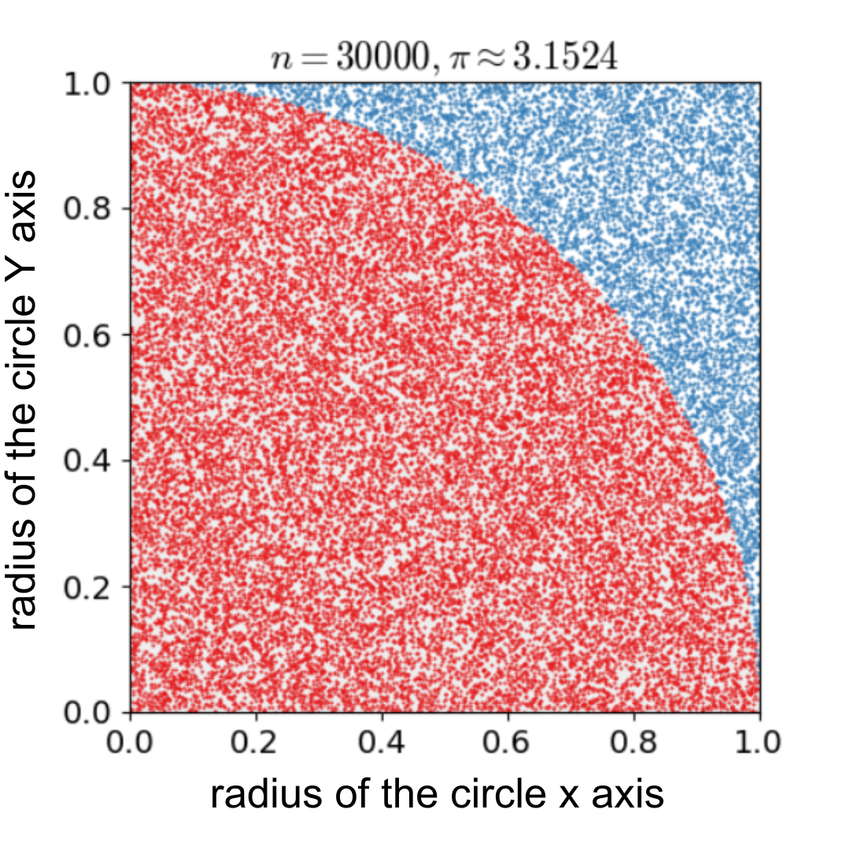
\includegraphics[scale=0.25]{Pi_MC.png}
    \caption{Graphical representation of $\pi$ estimation using the simple direct Monte Carlo integration method.}
    \label{fig:MC_pi_estimation}
\end{figure}
The simplest way to show the direct sampling method for integrals is through the computation of $\pi$: suppose that we have a square of side 1 and, inside it, 
the quadrant of a circle (of radius 1). It is known from high school geometry that:
\begin{equation}
    \frac{\pi}{4}=\frac{1}{4}\frac{\pi(1)^2}{(1)^2}=\frac{1}{4}\frac{A_{\text{quadrant}}}{A_{\text{square}}},
\end{equation}
from which it follows that we can compute the value of $\pi$ from the ratio between the two areas.
We now express the areas in terms of integrals
\begin{equation}
    \frac{\pi}{4}=\frac{\int_{\text{circle}}dxdy}{\int_{\text{square}}dxdy}=\int_{\text{square}}f(x,y)p(x,y)dxdy,
\end{equation}
with
\begin{equation}
    p(x,y)=\frac{1}{\int_{\text{square}}dxdy}
\end{equation}
and $f(x,y)$ defined in the following way:
\begin{equation}
    f(x,y)=
    \begin{cases}
    1,\hspace{1cm}\text{if }\sqrt{x^2+y^2}<1\\
    0,\hspace{1cm}\text{otherwise}.    
    \end{cases}
\end{equation}
Since $p(x,y)$ is non-negative and normalized, it can be treated as a probability distribution. We can thus say that
\begin{equation}
    \frac{\pi}{4}\approx \frac{1}{N}\sum_{i=1}^N f(x_i,y_i),
\end{equation}
the obtained result can be interpreted visually considering that we are filling the total area of the square with randomly distributed dots 
and counting how many of them end inside the circle compared to the total.\\
This simple method can be used (at least in theory) to compute every possible integral, nevertheless using a uniform distribution may 
result impractical when estimating functions that have sharp peaks: in this case most of the guesses made end up "outside" the region of interest 
and do not contribute to the estimation of the integral. Of course, this problem becomes more and more relevant the more dimensions we have.\\
In these cases, it is appropriate to use as a probability function that has a similar shape with respect to the target function we want to 
integrate, consider the following one-dimensional case:
\begin{equation}
    I=\int_{a}^{b}f(x)dx,
\end{equation}
where $f(x)$ has a sharp peak in a limited interval between $a$ and $b$ and is close to 0 everywhere else. Operating in the same 
way as before we obtain the following expression:
\begin{equation}
    I=\int_{a}^{b}\frac{f(x)}{p(x)}p(x)dx,
\end{equation}
and we can approximate the integral as
\begin{equation}
    I\approx I_N=\frac{1}{N}\sum_{i=1}^N\frac{f(x_i)}{p_(x_i)},
\end{equation}
while the variance of our estimation is found as 
\begin{equation}
    s^2=\frac{1}{N}\sum_{i=1}^N\left[\frac{f(x_i)}{p(x_i)}\right]^2-\left[\frac{1}{N}\sum_{i=1}^N\frac{f(x_i)}{p(x_i)}\right]^2,
\end{equation}
analyzing the expression for the variance estimator it becomes clear that it is minimized if $p(x)$ is chosen to be as close as 
possible to the target function $f(x)$, with the best result $s^2=0$ obtained for $p(x) = cf(x)$ (which would mean that it is possible to analytically 
integrate $f(x)$). This means that with a careful choice of the probability distribution it is possible to minimize the statistical fluctuations 
of our estimate and thus obtain the same accuracy with a smaller number of samples $N$.\\
Since multiple algorithms have been studied in order to build pseudonumber generators in the interval $(0,1)$ that are efficient, provide long periods 
for sequences of values and have uniform distribution in $n$-dimensional spaces (for example the Mersenne-Twister algorithm, used in this thesis \cite{matsumoto1998mersenne}), 
it is important to find ways to sample from other more complex (continuous) distributions $p(x)$, the easiest way to do so is through \textbf{CDF inversion} 
(cumulative density function inversion), which, as the name suggests, can be used when the analytical form of the cumulative distribution 
$P(x)$ is known.\\
Choosing for example the exponential distribution 
\begin{equation}
    \exp{\left(x;\lambda\right)}=\lambda e^{-\lambda x}\hspace{1cm}\text{for}\hspace{0.2cm}x>0, 
\end{equation}
for which we can obtain the expression for the cumulative density function easily:
\begin{equation}
    P(x)=\int_{0}^{x}\lambda e^{-\lambda x}dx = 1-e^{-\lambda x}.
\end{equation}
We now solve for $x$ to obtain
\begin{equation}
    x=-\frac{1}{\lambda}\log{(1-P(x))}.
\end{equation}
Since by definition the image of $P(x)$ is $[0,1]$, we can substitute it in the equation with the standard uniform random variable defined 
in $[0,1]$ $r$:
\begin{equation}
    x=-\frac{1}{\lambda}\log{(1-r)},
\end{equation}
and we obtain a random variable $x$ that follows the exponential distribution $p(x;\lambda)$.
\subsection{Markov Chain Monte Carlo}
The procedure illustrated in the previous section only works when an analytical expression for the cumulative distribution exists, 
this is not true in general and a different method is thus needed for a general distribution $p(x)$. To this scope \textbf{Markov chains} are 
used.\\
Let us define the random vector $\mathbf{X}$ as a sequence of $n$ random samples that are drawn one after the other:
\begin{equation}
    \mathbf{X}=\left(X_1,X_2,...,X_n\right),
\end{equation}
we call this vector an uncorrelated chains if each one of the variables $x_i$ are independent and thus uncorrelated, the probability of 
obtaining the chain $\mathbf{X}$ is then given by the product of the individual elements of the chain:
\begin{equation}
    P_n(\mathbf{X})=P_1(X_1)P_2(X_2)\cdots P_n(X_n).
\end{equation}
In a Markov chain this is not true and the random samples are correlated: a sequence of samples is said to be Markovian if the conditional 
probability of each sample of the sequence satisfies
\begin{equation}
    P(X_i|X_{i-1}...X_1)=P(X_i|X_{i-1}).
\end{equation}
This means that the probability of $X_i$ only depends on the previous element $X_{i-1}$ (and nothing else), with the exception of the first 
element of the chain. From this it follows that the order of the variables is important in the determination of the probability 
of the full random vector:
\begin{equation}
    P_n(X_1,X_2,...,X_n)=P_1(X_1)P(X_2|X_1)\cdots P(X_n|X_{n-1})
\end{equation}
where $P(X_i|X_{i-1})$ is the transition probability from $X_{i-1}$ to $X_i$.
We define $p_i^{(1)}$ ($\sum_i p_i^{(1)}=1$) the initial probability and $P(X_i|X_j)=P_{ij}$ the transition probability from $j$ to $i$. The transition 
probabilities are normalized for each $j$ such that $\sum_i P_{ij}=1$, in this way for every $k$ step $\sum_k p_i^{(k)}=1$ is obtained (note that, in continuous 
distribution, the sum is replaced by an integral).\\
Apart from the (obvious) normalization constraint, the single probabilities $p_i^{(k)}$ at the step $k$ (which are steps in time) are in 
general different from the probabilities $p_i^{(k-1)}$, the important mathematical result that is obtained under very general assumptions is that, 
after a necessary relaxation time that is different from system to system, the distribution relaxes to a stationary state $p_i$ which satisfies the 
relation
\begin{equation}
    p_i=\sum_{j}P_{ij}p_j
\end{equation}
for every $k$ step in the simulation.\\
The conditions required for this to happen are:
\begin{itemize}
    \item \textbf{connectedness}: every configuration of the distribution that we want to obtain must be accessible from any other configuration of the system in a finite number of steps.
    \item \textbf{no periodicity}: which means that, after having visited a specific configuration, it must be false that the same configuration will be accessible again only after 
    $nk$ steps with $n$ positive integer and $k$ fixed.
\end{itemize}
A Markov chain that satisfies these two conditions is called \textbf{ergodic} \cite{gubernatis2016quantum}.\\
Since the objective is to obtain a target stationary distribution $p_i$, we need a mean to do so starting from a more generic distribution (such as the uniform distribution 
in $[0,1]$), which means that a specific expression for the transition probabilities $P_{ij}$ is needed. The solution proposed 
by Metropolis \cite{metropolis1953equation} is to require the following relation for the transition probability $P_{ij}$ to be true:
\begin{equation}
    P_{ij}p_j=P_{ji}p_i,
    \label{detailed_balance_condition}
\end{equation}
which is the \textbf{detailed balance condition}. This means that the probability of transitioning from $j$ to $i$ is the same as 
the probability of transitioning from $i$ to $j$. This relation can be demonstrated using the \textbf{Master equation}:
\begin{equation}
    p_i^{(k)}-p_{i}^{(k-1)}=-\sum_{j}P_{ji}p_{i}^{(k-1)}+\sum_{j}P_{ij}p_{j}^{(k-1)},
    \label{master_equation}
\end{equation}
the stationary condition is obtained for
\begin{equation}
    p_i^{(k)}=p_{i}^{(k-1)}=p_i,
\end{equation}
From this it follows that 
\begin{equation}
    \sum_jP_{ji}p_i=\sum_jP_{ij}p_j,
\end{equation}
for every $i$, $j$ pair.\\
An obvious solution to this equation is found if \ref{detailed_balance_condition} holds.\\
%Let us now go to the continuous case, we substitute $p_i$ with $p(X)$ with $X$ configuration, $p_j$ with $p(X')$ and $P_{ij}$ with 
%$P(X,X')$. The detailed balance condition becomes:
%\begin{equation}
%    P(X',X)p(X)=P(X,X')p(X'),
%\end{equation}
%we now recast the transition probability $P(X,X')$ in the form 
%\begin{equation}
%    P(X',X)=\omega_{XX'}A_{XX'},
%\end{equation}
%with $A_{XX'}$ acceptance probability, which has a value between 0 and 1 for each couple $X$ and $X'$, and $\mathbf{\omega}$ symmetric matrix 
%($\omega_{XX'}=\omega_{X'X}$), with values between 0 and 1 and with the property $\Sigma_{X'}\omega_{XX'}=1$.\\
%If we substitute this form for the transition probability in the detailed balance equation we obtain
%\begin{equation}
%    \frac{A_{XX'}}{A_{X'X}}=\frac{p(X')}{p(X)},
%\end{equation}
We now recast the transition probability matrix $P_{ij}$ in the form
\begin{equation}
    P_{ij}=T_{ij}A_{ij},
\end{equation}
where $T_{ij}$ is the symmetric matrix $(T_{ij}=T_{ji})$ of the trial transition proposal probabilities with the additional properties 
$0\le T_{ij}\le 1$ and $\Sigma_i T_{ij}=1$, while $A_{ij}$ are the elements of the acceptance matrix, whose form is 
\begin{equation}
    A_{ij}=\min{\left\{1,\frac{p_i}{p_j}\right\}}\hspace{1cm}i\neq j.
\end{equation}
Using this configuration we can show that the condition of detailed balance is obeyed by assuming $p_i<p_j$ (we are not posing any constraint 
on the system by doing this since the choice of the indices is arbitrary) and observing that
\begin{equation}
    P_{ij}=T_{ij}\frac{p_i}{p_j}=T_{ji}\frac{p_i}{p_j}=T_{ji}\cdot 1\cdot\frac{p_i}{p_j}=P_{ji}\frac{p_i}{p_j},
\end{equation}
from which \ref{detailed_balance_condition} follows.\\
The complete algorithm, known as the \textbf{Metropolis algorithm}, proposes a new $i$ state given the present $j$ with trial transition 
probability $T_{ij}$, then uses the $A_{ij}$ elements of the acceptance matrix to accept $i$ or reject it (and thus keep $j$). Whether the new $i$ state 
is accepted or rejected depends on the uniform random variable defined in $[0,1]$ $r$: if $r<A_{ij}$ $i$ is accepted, otherwise it 
is rejected.
\begin{figure}[H]
    \centering
    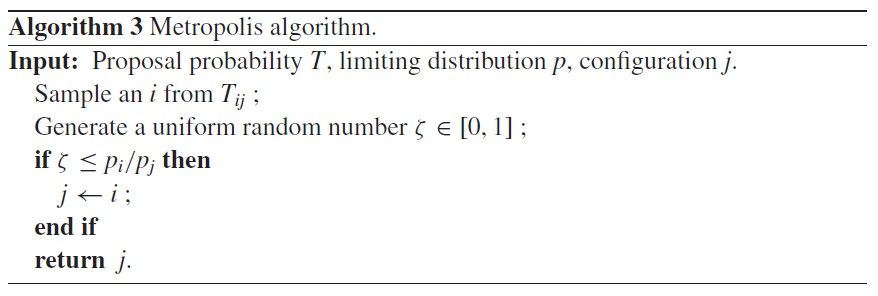
\includegraphics[scale=0.8]{Metropolis_algo.jpg}
    \caption{Schematic representation of the Metropolis algorithm procedure \cite{gubernatis2016quantum}.}
    \label{fig:Metropolis}
\end{figure}
It is possible to generalize the algorithm to one that does not have a symmetric trial transition probability matrix $T_{ij}$:
given a generic acceptance ratio $R_{ij}$ such that $A_{ij}=\min\left\{1,R_{ij}\right\}$ defined as
\begin{equation}
    R_{ij}=\frac{S_{ij}}{1+\frac{T_{ij}p_j}{T_{ji}p_i}},
\end{equation}
with $S_{ij}$ non-negative symmetric matrix, if $S_{ij}$ is chosen to be:
\begin{equation}
    S_{ij}=
    \begin{cases}
        1+\frac{T_{ji}p_i}{T_{ij}p_j},\hspace{1cm}T_{ij}p_j\ge T_{ji}p_i,\\
        1+\frac{T_{ij}p_j}{T_{ji}p_i},\hspace{1cm}T_{ji}p_1\ge T_{ij}p_j,
    \end{cases}
\end{equation}
the \textbf{Metropolis-Hasting algorithm} is obtained with acceptance ratio $R_{ij}$:
\begin{equation}
    R_{ij}=\frac{T_{ji}p_i}{T_{ij}p_j}.
    \label{metropolis-hastings_discrete}
\end{equation}
In the special case where we want to obtain a random variable $X$ distributed as a generic continuous function $f(x)$ (not necessarily 
normalized) using as a prior distribution a known distribution $h(x)$, we may identify the trial transition probability from a state $x$ to 
a state $x'$ with
\begin{equation}
    T_{x'x}=\pi(x')dx
\end{equation}
independent on the current state $x$, the acceptance ratio $R_{x'x}$ then becomes
\begin{equation}
    R_{x'x}=\frac{T_{xx'}p_{x'}}{T_{x'x}p_{x}}=\frac{\pi(x)dxf(x')dx}{\pi(x')dxf(x)dx}=\frac{\pi(x)f(x')}{\pi(x')f(x)},
    \label{metropolis-hastings-continuous}
\end{equation}
with acceptance probability $A_{x'x}$:
\begin{equation}
    A_{x'x}=\min{\left\{1,\frac{\pi(x)f(x')}{\pi(x')f(x)}\right\}}.
    \label{acceptance_prob_distrib}
\end{equation}
Using the above formulation (easily generalizable at least in theory to $N$ dimensions) it is possible to sample random variables from any generic continuous 
unnormalized function. The main drawbacks of this method are the fact that a relaxation to the stationary distribution is necessary (and the number of steps required is 
not known a priori) and that the obtained samples are correlated.
\subsection{Diagrammatic Quantum Monte Carlo}
In Chapter 2 we have seen that the polaron model can be solved by perturbatively expanding the related Green's function (which is a 
solution to the equation of motion of the system) in the imaginary time formalism. Since the Green's function in this formalism can be cast 
in a form that makes it real and non-negative, it can be sampled as if it were a distribution using the methods provided by Markov Chain Monte Carlo.\\
To this objective, we need a method to ergodically represent all the possible configurations of the polaron system. This approach can be used in many different condensed 
matter physics systems where a similar expansion is possible, provided that the weight of negative diagrams (which in our specific case do not appear, but are generally present in fermionic 
systems) does not hinder the accuracy of the estimated quantity \cite{gull2011continuous}.\\
Given a function represented as \ref{GF_polaron_series} (without the minus sign) it is possible to sample it as a distribution $Q(\left\{y\right\})$ 
which depends on a set of variable $y$:
\begin{equation}
    Q(\left\{y\right\})=\sum_{n=0}^{+\infty}\sum_{\xi_n}\int dx_1 \cdots \int dx_n D_n(\xi_n,{y},x_1,...,x_n),
\end{equation}
with $\{y\}$ external variables and $\{x_i\}$ internal variables (to be integrated out).\\
Using the Metropolis-Hastings algorithm it is possible to sample variables from this distribution and in the limit of a large number of 
samples retrieve the full function up to a normalization constant $C$ with no approximations:
\begin{equation}
    Q_i(\{y\})=C\hspace{0.2cm} G(\mathbf{k},\tau).
\end{equation}
The fundamental difference with respect to an usual Monte Carlo integration is the fact that the parameter space of internal variables 
varies between different iterations of the simulation: ways to model transitions between these different states together with the correct trial transition probability 
are required.\\
In order to do so, a number of elementary updates are defined such that there are at least enough to satisfy the ergodicity requirement \cite{gubernatis2016quantum} for the 
Markov chain which relaxes to the target distribution (the system under study). The Metropolis-Hastings algorithm in DMC uses as acceptance probabilities for transitions 
between two different states characterized by the variables $i=\left\{y_i,\xi_i,\mathbf{x}_i\right\}$ and $i=\left\{y_j,\xi_j,\mathbf{x}_j\right\}$ respectively the relative weight of the two 
diagrams.\\
In fact, given the two diagrams $D_{n_i}(i)$ and $D_{n_j}(j)$ (which may be different in the value of one or more variables, whether internal or external, and more importantly in the \textit{number} 
of internal variables if the rank of the two diagrams is different), the acceptance ratio $R_{ij}$ is proportional to:
\begin{equation}
    R_{ij}\propto \frac{D_{n_i}(i)}{D_{n_j}(j)}= \frac{C\hspace{0.2cm}D_{n_i}^*(i)}{C\hspace{0.2cm}D_{n_j}^*(j)}=\frac{D_{n_i}^*(i)}{D_{n_j}^*(j)},
\end{equation}
where the $D_{n_k}^*(k)$ are the properly normalized weights, different from the weights of the generated distribution up to a normalization constant \cite{HahnThomas2017DqMC}.\\
When negative-valued diagrams are present, the acceptance ratio is performed on the absolute values of the weights. Operating in this way, however, we expose ourselves 
to the \textbf{negative sign problem}: when we want to compute an observable $O$ from the Monte Carlo simulation, whether it be the (normalized) distribution 
or any other quantity of interest, we must take into account the negative weights:
\begin{equation}
    O = O_N =\left(\frac{1}{N}\sum_{i=1}^N |O_i(D(i))|\right)\left(\frac{N^+-N^-}{N}\right)^{-1}=\frac{1}{N^+-N^-}\sum_{i=1}^N |O_i(D(i))|,
\end{equation}
and the variance of the Monte Carlo estimate diverges for $N^+ - N^-\approx 0$.\\
Two basic classes of elementary updates can be recognized \cite{van2010diagrammatic}\cite{mishchenko2000diagrammatic}:
\begin{itemize}
    \item \textbf{class I updates}: they change one or more variables (internal or external), the new variables $\mathbf{x}$ are proposed using a suitable
    distribution $\pi(\mathbf{x})$ (some distribution might be more suited than others depending on the specific system), and the acceptance ratio is computed using 
    the standard Metropolis-Hastings algorithm (\ref{metropolis-hastings_discrete} and \ref{metropolis-hastings-continuous} depending on the type of variable and prior 
    distribution)
    \item \textbf{class II updates}: in this class of updates the order of the diagram is changed, and thus the number of internal variables is increased or 
    reduced. Considering an update where the order of the diagram is increased, the new $m$ internal variables are sampled from a distribution $\rho(\mathbf{x})$ 
    and the acceptance ratio $R_{ij}$ is computed as follows:
    \begin{equation}
        R_{ij}=\frac{p_A}{p_B}\frac{D_{n_i=n_j+m}(i)}{\rho(x_1,...,x_n)D_{n_j}(j)},
    \end{equation}
    where $p_A$ and $p_B$ are the so-called \textbf{context factors} that take into account the ways it is possible to transition from state $A$ to 
    state $B$ and thus depend on how the processes are organized (it does not usually reduce to the simple relation $p_A/p_B=1$) \cite{fehske2007computational}. The 
    opposite process which reduces the order of the diagram from $n$ to $n-m$ is found to be 
    \begin{equation}
        R_{ji}=\frac{1}{R_{ij}},
    \end{equation}
    in agreement with the detailed balance requirement.
\end{itemize}
Employing these rules and carefully crafting prior distributions and acceptance ratios, it is possible to sample a distribution that is 
equal up to a normalization constant a Green's function in imaginary time formalism, provided that it can be expanded in a similar way to \ref{GF_polaron_expansion_00}.
\begin{figure}[H]
    \centering
    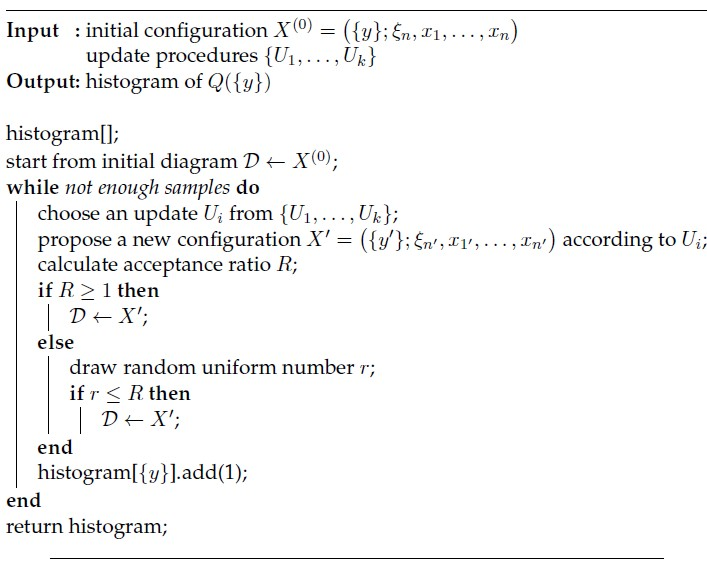
\includegraphics[scale=0.8]{Diag_MC_algo.jpg}
    \caption{Diagrammatic Monte Carlo algorithm procedure \cite{HahnThomas2017DqMC}.}\
    \label{fig:diag_MC_algo}
\end{figure}
The specific updates, however, greatly vary between different systems considering issues such as ergodicity requirements, context factors and the sign problem.
